\documentclass[xcolor={dvipsnames,svgnames,table}]{beamer}

\usepackage{slides}
\usepackage{tikz}
\usepackage{python}

\usetikzlibrary{calc}
\usetikzlibrary{positioning}

\newcommand{\bankdistance}{4}
\tikzstyle{bank}=[
  draw,
  minimum width=1.5cm,
  minimum height=1cm,
  font=\huge
]
\tikzstyle{op}=[
  ->,
  ultra thick
]

\newcommand{\drawbanks}[6]{{
  \newcommand{\banka}{#1}
  \newcommand{\bankb}{#2}
  \newcommand{\bankaa}{#3}
  \newcommand{\bankbb}{#4}
  \newcommand{\bankaaa}{#5}
  \newcommand{\bankbbb}{#6}

  \node[bank, label=above:{Replica $A$}] (a1) at (0,              0) {\banka};
  \node[bank                           ] (a2) at (0,             -3) {\bankaa};
  \node[bank                           ] (a3) at (0,             -6) {\bankaaa};
  \node[bank, label=above:{Replica $B$}] (b1) at (\bankdistance,  0) {\bankb};
  \node[bank                           ] (b2) at (\bankdistance, -3) {\bankbb};
  \node[bank                           ] (b3) at (\bankdistance, -6) {\bankbbb};

  \draw[op] (a1) -- (a2);
  \draw[op] (a2) -- (a3);
  \draw[op] (b1) -- (b2);
  \draw[op] (b2) -- (b3);
}}

\newcommand{\zigzag}[2]{{
  \newcommand{\banka}{#1}
  \newcommand{\bankb}{#2}

  \draw[red, op] ($(\banka) + (0, -0.7)$) -- ($(\bankb) + (0, -1.0)$);
  \draw[red, op] ($(\bankb) + (0, -1.0)$) -- ($(\banka) + (0, -1.3)$);
  \draw[red, op] ($(\banka) + (0, -1.3)$) -- ($(\bankb) + (0, -1.6)$);
  \draw[red, op] ($(\bankb) + (0, -1.6)$) -- ($(\banka) + (0, -1.9)$);
}}

\newcommand{\dbs}{\mathcal{D}}
\newcommand{\var}{\textsf{Var}}
\newcommand{\ints}{\mathbb{Z}}

\newcommand{\wimp}{W$\iinvariant$MP}
\newcommand{\imp}{$\iinvariant$MP}
\newcommand{\impaexp}{\textsf{Aexp}}
\newcommand{\impbexp}{\textsf{Bexp}}
\newcommand{\impcom}{\textsf{Com}}
\newcommand{\impskip}{\textsf{skip}}
\newcommand{\impif}[3]{\textsf{if}(#1)\set{#2}\textsf{else}\set{#3}}

\newcommand{\iinvariant}{\mathcal{I}}
\newcommand{\iconfluent}{$\iinvariant$-confluent}
\newcommand{\iconfluence}{$\iinvariant$-confluence}
\newcommand{\ipreservation}{$\iinvariant$-preservation}
\newcommand{\ipreserving}{$\iinvariant$-preserving}
\newcommand{\isafety}{$\iinvariant$-safety}
\newcommand{\isafe}{$\iinvariant$-safe}
\newcommand{\istrength}{$\iinvariant$-strength}
\newcommand{\istrong}{$\iinvariant$-strong}
\newcommand{\istrengthstar}{\istrength$^\ast$}
\newcommand{\istrongstar}{\istrong$^\ast$}
\newcommand{\iconvergence}{$\iinvariant$-convergence}
\newcommand{\iconvergent}{$\iinvariant$-convergent}


\title{Enforced \iconfluence{}}
\author{Michael Whittaker}
\date{December 12, 2016}

\begin{document}
\begin{frame}
  \maketitle
\end{frame}

\begin{frame}{Coordinating}
  \begin{center}
    \begin{tikzpicture}
      \drawbanks{\$50}{\$50}
                {\$60}{\$60}
                {\$80}{\$80}

      \draw[op] ($(a1) + (-2, 0)$) -- (a1) node[midway, above] {$+\$10$};
      \draw[op] ($(b1) + (+2, 0)$) -- (b1) node[midway, above] {$+\$20$};
      \draw[op] (a2) -- ($(a2) + (-2, 0)$) node[midway, above] {OK};
      \draw[op] (b3) -- ($(b3) + (+2, 0)$) node[midway, above] {OK};

      \zigzag{a1}{b1}
      \zigzag{a2}{b2}
    \end{tikzpicture}
  \end{center}
\end{frame}

\begin{frame}{Coordinating}
  \begin{center}
    \begin{tikzpicture}
      \drawbanks{\$50}{\$50}
                {\$20}{\$20}
                {\$20}{\$20}

      \draw[op] ($(a1) + (-2, 0)$) -- (a1) node[midway, above] {$-\$30$};
      \draw[op] ($(b1) + (+2, 0)$) -- (b1) node[midway, above] {$-\$40$};
      \draw[op] (a2) -- ($(a2) + (-2, 0)$) node[midway, above] {OK};
      \draw[op] (b3) -- ($(b3) + (+2, 0)$) node[midway, above] {NO};

      \zigzag{a1}{b1}
      \zigzag{a2}{b2}
    \end{tikzpicture}
  \end{center}
\end{frame}

\begin{frame}{Avoiding Coordination}
  \begin{center}
    \begin{tikzpicture}
      \drawbanks{\$50}{\$50}
                {\$60}{\$70}
                {\$80}{\$80}

      \draw[op] ($(a1) + (-2, 0)$) -- (a1) node[midway, above] {$+\$10$};
      \draw[op] ($(b1) + (+2, 0)$) -- (b1) node[midway, above] {$+\$20$};
      \draw[op] (a2) -- ($(a2) + (-2, 0)$) node[midway, above] {OK};
      \draw[op] (b2) -- ($(b2) + (+2, 0)$) node[midway, above] {OK};

      \draw[dashed, op] (a2) -- (b3) node[near start, sloped, above] {$+\$10$};
      \draw[dashed, op] (b2) -- (a3) node[near start, sloped, above] {$+\$20$};
    \end{tikzpicture}
  \end{center}
\end{frame}

\begin{frame}{Avoiding Coordination}
  \begin{center}
    \begin{tikzpicture}
      \drawbanks{\$50}{\$50}
                {\$20}{\$10}
                {-\$20}{-\$20}

      \draw[op] ($(a1) + (-2, 0)$) -- (a1) node[midway, above] {$-\$30$};
      \draw[op] ($(b1) + (+2, 0)$) -- (b1) node[midway, above] {$-\$40$};
      \draw[op] (a2) -- ($(a2) + (-2, 0)$) node[midway, above] {OK};
      \draw[op] (b2) -- ($(b2) + (+2, 0)$) node[midway, above] {OK};

      \draw[dashed, op] (a2) -- (b3) node[near start, sloped, above] {$-\$30$};
      \draw[dashed, op] (b2) -- (a3) node[near start, sloped, above] {$-\$40$};
    \end{tikzpicture}
  \end{center}
\end{frame}

\begin{frame}{\iconfluence{}}
  \begin{columns}
    \begin{column}{0.5\textwidth}
      \frame{
        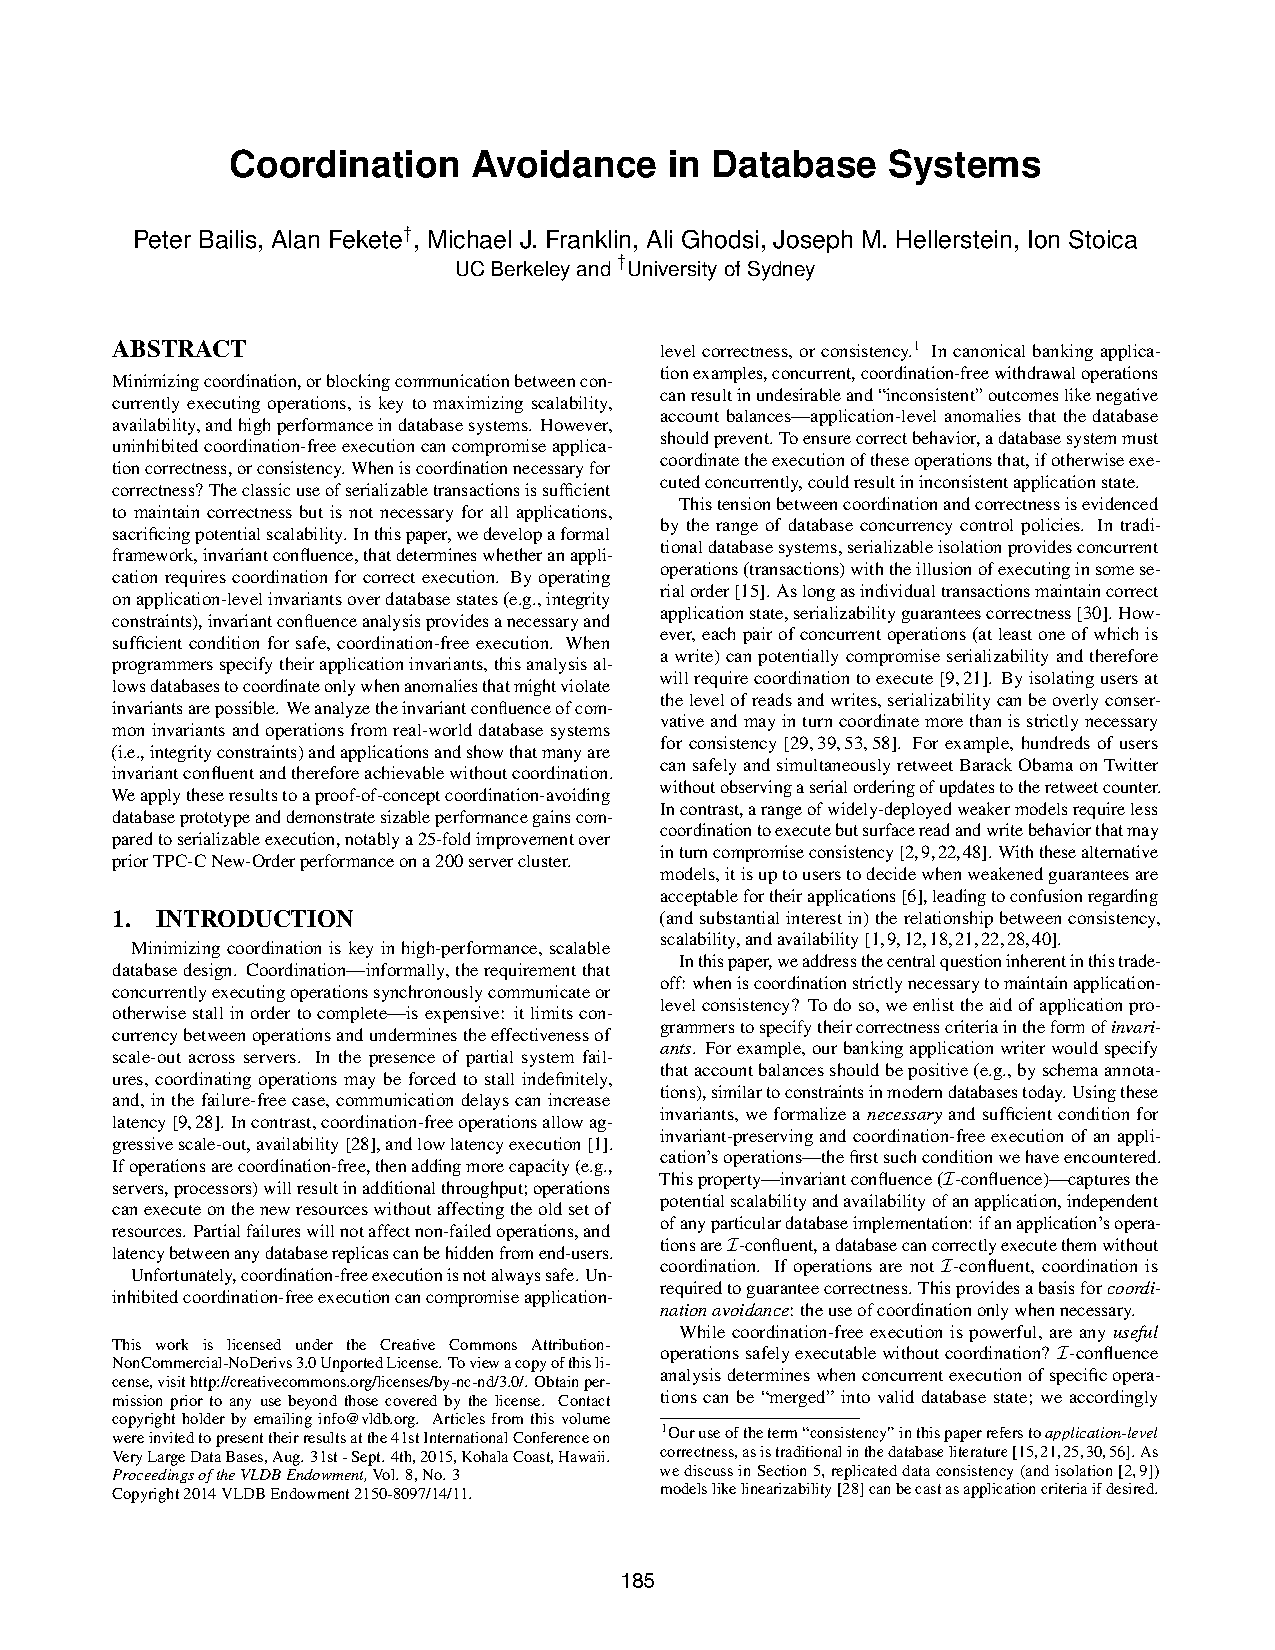
\includegraphics[width=\textwidth]{figs/bailis-iconfluence-page1.pdf}
      }
    \end{column}
    \begin{column}{0.5\textwidth}  %%<--- here
      \begin{center}
        A set of of transactions $T$ is \emph{invariant-confluent}
        (\iconfluent) with respect to $I$ if and only if $T$ can execute
        without coordination while preserving $I$.
      \end{center}
    \end{column}
  \end{columns}
\end{frame}

\begin{frame}{\iconfluence{}}
  \begin{center}
    \begin{tikzpicture}
      \newcommand{\proofa}{proof17}
      \newcommand{\proofb}{proof12}
      \newcommand{\proofc}{proof16}
      \newcommand{\proofwidth}{5cm}

      \node[draw, fill=white] (\proofa) at (0, 0) {
        \includegraphics[width=\proofwidth]{figs/\proofa.pdf}
      };
      \node[draw, fill=white] (\proofb) at (\proofa.south east) {
        \includegraphics[width=\proofwidth]{figs/\proofb.pdf}
      };
      \node[draw, fill=white] (\proofc) at (\proofb.south east) {
        \includegraphics[width=\proofwidth]{figs/\proofc.pdf}
      };
    \end{tikzpicture}
  \end{center}
\end{frame}

\begin{frame}[fragile]{Vision}
  \begin{center}
    \begin{Python}[gobble=6]
      x = PNCounter(0)

      set_invariant(x >= 0)

      # Good!
      @transaction
      def foo():
        x.increment(42)

      # Bad!
      @transaction
      def bar():
        x.decrement(1)
    \end{Python}
  \end{center}
\end{frame}

\begin{frame}[fragile]{Vision}
  \begin{center}
    \begin{Python}[gobble=6]
      employees = Map[Int, String]()
      teams = Set[Set[Int]]

      # All ids in teams must appear in employees.
      set_invariant(forall team in teams.
        team subset employees.keys())
      # All teams must be disjoint.
      set_invariant(forall a, b in teams.
        a != b => a intersect b = {})
      # Every employee must be on a team
      set_invariant(union(teams) = employees.keys())

      @transaction
      def add_employee(name):
        id = employees.unique_id()
        employees.put(name, id)
        teams[0].add(id)
    \end{Python}
  \end{center}
\end{frame}

\begin{frame}
  - formalism accompanied with informal explanaation
  - formalize question
\end{frame}

\begin{frame}
  - geometric interpretation with pictures
\end{frame}

\begin{frame}
  - examples
  - increment
  - decrement
  - x = y with incremenet/decrement
  - cross with +x
  - cross with +y
  - cross with +x, +y
  - single point
\end{frame}

\begin{frame}
  - one is enough with picture
\end{frame}

\begin{frame}
  - solution
  - say its implemented
\end{frame}

\end{document}
